\section{Methodology}

This section details the process in developing a program to optimise the performance of PV and solar-thermal hybrid systems for a building, using a genetic algorithm. First, the method by which data was collected is discussed. The equations to be implemented are laid out below, before the genetic algorithm is introduced and discussed in detail, including fitness function, constraint function, and options function. The section is concluded by discussing the limitations of this program and recommendations of how it can be improved upon are detailed.

\subsection{Data Collection}

\subsubsection{Demand Data}

Electrical and heating demand data is collected from various sources. The demand data is sourced directly from Heriot-Watt University Estates Service \cite{HWES}. This data is initially given in monthly format. It is required to have it in hourly format so the average value for a day is taken for each separate month. This daily average is then interpolated alongside a general load profile for a day to create the load profile for the building.

\begin{figure}[h!]
	\centering
    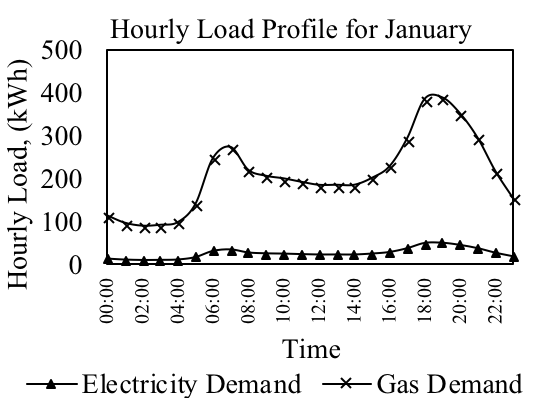
\includegraphics[width=1\hsize]{Figures/LoadProfiles.png}
    \caption{Interpolated hourly load profile for both electricity and gas demand. Adapted from monthly data  \cite{HWES}}
    \label{fig:LoadProfiles}
  \end{figure}
  
  \subsubsection{Resource Data}
  
  Hourly direct and global radiation data is taken from PVGIS \cite{PVGIS} for the location of the building. The same data is also acquired from the Australian Renewable Energy Mapping Infrastructure \cite{AREMI} for a location with stronger irradiance which is used to draw comparisons and conclusions. This data is imported and vectorised in Matlab.
  
  \subsection{Energy Balance}
  
 Equations for PV panels, flat-plate collectors, battery charge/discharge and the two objectives of minimising consumer cost and maximising the CO\textsubscript{2} reduction are required. These are laid out below.
 
\subsubsection{Photovoltaic}

\begin{equation}
E_{PV} = N_{PV} \ A_{PV} \ I_{G} \ \eta_{PV}
\end{equation}
\newline
Where:\newline
E\textsubscript{PV} = Electricity output from the PV array;\newline
N\textsubscript{PV} = Number of PV panels;\newline
A\textsubscript{PV} = Area covered by one PV panel;\newline
I\textsubscript{G} = Global radiation present at the location;\newline
$\eta _{PV}$ = Solar panel efficiency.\newline

Eq. 1 shows the electricity output from the PV array. This equation is based on the panels being horizontal. If the panels were being installed on a tilted roof, this would change.

\subsubsection{Solar Thermal}

\begin{equation}
Q_U = F_R \tau \alpha \ A_{ST} \ I_D \ - \ F_R U_L \ A_{ST} \ (T_{in} - T_{amb})
\end{equation}
\newline
Where:
$Q_U$ = The useful heat energy generated by the array of solar thermal panels;\newline
$F_R \tau \alpha$ = A constant relating to transmittance and absorbance of the panel being used;\newline
$A_{ST}$ = The area covered by one solar thermal panel;\newline
$I_D$ = Direct radiation received by the panels from the sun;\newline
$F_R U_L$ = A constant for the specific panel being used;\newline
$T_{in}$ = Temperature of the fluid within the panel;\newline
$T_{amb}$ = Ambient temperature, 25{\degree}C. \newline

Eq. 2, shows the useful heat output generated by the ST array. This equation is based on a flat plate collector, and therefore is not valid for tube collectors.

\subsubsection{Heat Storage}

if $Q_{U_{n+1} \ > \ Q_{D_{n+1}}}$:

\begin{equation}
Q_{T_{n+1}} = Q_{T_n} \ + (\ Q_{U_{n+1}} \ - \ Q_{D_{n+1}}) 
\end{equation}

Else If $Q_{U_{n+1}} \ < \ Q_{D_{n+1}}$ \newline

\hspace*{15pt} \vspace*{2pt} And $Q_{T_n} \ \geq \ Q_{D_{n+1}} \ - \ Q_{U_{n+1}}$:

\begin{equation}
Q_{T_{n+1}} =Q_{T_{n}} \ + \ (Q_{U_{n+1}} \ - \ Q_{D_{n+1}})
\end{equation}

\hspace*{15pt} Else 
\begin{equation}
Q_{T_{n+1}} = 0
\end{equation}

Else 
\begin{equation}
Q_{T_{n+1}} = Q_{T_{n}}
\end{equation}
\newline
Where:
n = Previous timestep;\newline
n+1 = Current timestep;\newline
$Q_D$ = Heating demand;\newline
$Q_T$ = thermal storage level.\newline
\newline
Eq. 3,4,5 and 6 are for thermal storage. This states that when the useful heat energy generated is larger than the demand, the excess will be stored. If the demand is larger than the generation, then the stored energy will be used to cover the excess demand. 

\subsubsection{Electrical Storage}

if $E_{PV_{n+1} \ > \ E_{D_{n+1}}}$:

\begin{equation}
E_{B_{n+1}} = E_{B_n} \ + (\ E_{PV_{n+1}} \ - \ E_{D_{n+1}}) 
\end{equation}

Else If $E_{PV_{n+1}} \ < \ E_{D_{n+1}}$ \newline

\hspace*{15pt} \vspace*{2pt} And $E_{B_n} \ \geq \ E_{D_{n+1}} \ - \ E_{PV_{n+1}}$:

\begin{equation}
E_{B_{n+1}} =E_{B_{n}} \ + \ (E_{PV_{n+1}} \ - \ E_{D_{n+1}})
\end{equation}

\hspace*{15pt} Else 
\begin{equation}
E_{B_{n+1}} = 0
\end{equation}

Else 
\begin{equation}
E_{B_{n+1}} = E_{B_{n}}
\end{equation}
\newline
Where:
$E_D$ = Electricity demand, W;\newline
$E_B$ = Electricity stored in the Li-Ion batteries;\newline
\newline
Eq. 7,8,9 and 10 describe the electricity storage system. It works in the same way as that of the thermal storage as described previously. 

\subsubsection{Performance Indicators}

\begin{equation}
S = \frac{1}{E_{out} \ s_{PV} + Q_{out} \ s_{ST}}
\end{equation}

\begin{equation}
C = N_{PV} \ c_{PV} \ + \ N_{ST} \ c_{ST} \ + \ c_B \ + \ c_T \ - \ c_s
\end{equation}
\newline
where: 
S = Total $CO_2$ saving in kg; \newline
$E_{out} = s_{PV} \ A_{PV} \ N_{PV} \ I_G  \ \eta_{PV}$;\newline
$Q_{out} = (s_{ST} (F_R \tau \alpha \ A_{ST} \ N_{ST} \ I_D ) \ - \ (F_R U_L \ A_{ST} \ N_{ST} \ (T_{in} - T_{amb})$; \newline
$s_{PV} = 0.482 \ kg \  \frac{CO_2}{kWh}$; \newline
$s_{ST} = 0.24 \ kg \ \frac{CO_2}{kWh}$; \newline
C = The consumer cost; \newline
$c_{PV}$ = Cost per panel \newline %%(210*0.77*1.2); [ref] 
$P_{PV}$ = Rated power output of the PV panel in kW.; \newline %%[ref]
$c_{ST}$ = Cost of the solar thermal panels in £/Unit \newline %%($900); [ref] 900*0.77*1.2
$c_B$ = Cost of the electrical storage system; \newline %%[ref]
$c_T$ = Cost of the heat storage system; \newline %%[ref]
$c_s$ = Total value of savings earned from tariffs. \newline

Eq. 11 and 12 are the performance indicators for the project. Eq. 11 is the total carbon dioxide saving in kg and Eq. 12 is the consumer cost. These two equations are the basis of what the GA is working towards finding the optimal solution to.

\subsection{Genetic Algorithm}

The built in genetic algorithm function within the Global Optimisation Toolbox for Matlab is used. It is tailored to fit the purpose. This program uses the function ‘GAMULTIOBJ’ \cite{GAMULTIOBJ} to perform the genetic algorithm on the multi-objective problem. This built-in function aims to minimise the two specified objectives. It does this through the use of the fitness function and constraint function as well as a specified set of options, including boundary conditions and number of variables.

\subsubsection{Fitness Function (Objective Function)} 
The fitness function takes the input data, and using the two objective function equations, as defined by the performance indicators earlier, calculates two vectors of data. This process is repeated using the new values for the variable.

\subsubsection{Constraint Function}
To ensure the solutions obtained from the genetic algorithm simulation are suitable, a constraint function is required. The constraint function in this case contains 3 separate constraints: The total area covered by both types of panels must not exceed the defined maximum area; the PV panels must meet a specified portion of the total electricity demand; the solar thermal panels must meet a specified portion of the total thermal demand required.

The following three equations are passed through as the constraint function, c:
 
\begin{equation}
N_{PV} \ A_{PV} \ + \ N_{ST} \ A_{ST} \ - \ A_{max}
\end{equation}

\begin{equation}
x E_D \ - \ E_{out}
\end{equation}

\begin{equation}
x Q_D \ - Q_{out}
\end{equation}

where x is the factor of the demand that must be met by the system for the Pareto front.

\subsubsection{Options}

The options function allows for plotting of the results in a Pareto plot, as well as allowing for the passing of all information required by the genetic algorithm. To obtain a sufficient amount of results on the Pareto front, a population size of 200 is implemented. Custom creation, mutation and crossover functions are also passed through using functions created by MathWorks \cite{matlabb}. This allowed for the final values for the number of PV panels, flat-plate collectors, Li-Ion batteries and PCM heat batteries to be given in integer form instead of the default real number format.

\subsection{Constant Values}

There are various constants used throughout the simulation. These values are defined as in Table \ref{Constants}. Depending on the model of the panels the areal, transmittance, absorbance and heat loss coefficient are all subject to change. This simulation only uses one of each panel type and therefore are constant here.

\begin{table}[H]
\caption{Summary of variables and constants with their values and definition.}
\vspace{5pt}
\label{Constants}
\centering
\begin{tabular}{@{}lll@{}}
\toprule
\textbf{Constant} & \textbf{Value} & \textbf{Definition} \\ \toprule
F$_R$U$_L$ & 3.4 & Heat loss coefficient \\ \midrule
F$_R$$\tau$$\alpha$ & 0.726 & Transmittance/Absorbance \\ \midrule
T$_{in}$ & 70\degree C & Temperature of collector. \\ \midrule
T$_{amb}$ & 25\degree C & Ambient temperature. \\ \midrule
A$_{ST}$ & 2.5m$^2$ & Flat-plate collector area. \\ \midrule
A$_{PV}$ & 1.91m$^2$ & PV panel area. \\ \midrule
A$_{max}$ & 1600m$^2$ & Maximum areal space. \\ \midrule
V$_B$ & 0.13m$^3$  & Li-Ion battery volume. \\ \midrule
V$_{TB}$ & 0.26m$^3$ & Heat battery volume. \\ \midrule
s$_{PV}$ & $0.482 \ kg \  \frac{CO_2}{kWh}$ & CO$_2$ savings from PV \cite{britgas}. \\ \midrule
s$_{ST}$ & $0.24 \ kg \  \frac{CO_2}{kWh}$ & CO$_2$ savings from ST \cite{britgas}. \\ \midrule
c$_{PV}$ & £186 & Cost of a PV panel \cite{irenaB}. \\ \midrule
c$_{ST}$ & £835 & Cost of a ST panel \cite{ecodirect} \\ \midrule
c$_B$ & £1540 & Cost of electrical storage \cite{irena}. \\ \midrule
c$_T$ & £2100 & Cost of thermal storage \cite{sunamp}. \\ \midrule
c$_s$ &£0.635/kW & UK gen. tariff \cite{EST1} \cite{EST2}. \\ \midrule
\end{tabular}
\end{table}

\subsection{Program Flow Chart}

The flow chart can be seen in Appendix A. It details the method by which the genetic algorithm will function. It takes the inputs of resource data, component data, constraints, boundaries, fitness function and options data and then implements the algorithm. Once it has completed the process, a check is done by the algorithm to see if the criteria have been met, if the criteria are not met, the algorithm will repeat until the solution is obtained.




 